\documentclass[11pt,a4paper]{article}

\usepackage[utf8]{inputenc}
\usepackage[T1]{fontenc}
\usepackage{lmodern}
\usepackage[english]{babel}
\usepackage{amsmath,amssymb}
\usepackage{icomma}
\usepackage[a4paper,margin=1.4cm]{geometry}
\usepackage{enumitem}
\usepackage{xcolor}
\usepackage[most]{tcolorbox}
\usepackage[hypertexnames=false]{hyperref}
\hypersetup{
	colorlinks=true,       % Enables link highlighting (removes borders)
	linkcolor=blue,        % Color of internal links (sections, table of contents)
	urlcolor=cyan,         % Color of Web Links (URLs)
	citecolor=green,       % Color of bibliographic citations
	pdftitle={SPM Tutorial Report},
	pdfauthor={AKABASSI J. G. O. W. Samuel}
}
\usepackage{float}

\setlength{\parskip}{0pt}
\setlength{\parindent}{0pt}


\begin{document}

\section*{Search Space}
\addcontentsline{toc}{section}{Search Space}

When applying DFS, the order in which the elements of the alphabet appear is significant. For this reason, the enumerated objects are sequences (the search space is a space of sequences). Furthermore, elements may be repeated, which is why the number of enumerated objects is infinite and the program does not terminate (until it is forcibly stopped by a $RecursionError$ exception).


\section*{Formula for N(m, d)}
\addcontentsline{toc}{section}{Formula for N(m, d)}

Let $m$ be the length of the alphabet. Let $d$, $k$, and $l$ be sequence lengths. Let $N_{k}$ be the number of sequences of length $k$. Let $N(m, d)$ be the total number of non-empty sequences of length at most $d$. We have the following formulas: $N_{k} = m^{k}$; $N(m, d) = \sum_{l=1}^{d} m^{l}$. Experimental measurements performed on the functions $compter$ and $generer$ confirmed the validity of these formulas, as can be seen in Figures \ref{fig:compter-vs-generer-sequence-count} and \ref{fig:compter-vs-generer-execution-time}.


\section*{Key Definitions}
\addcontentsline{toc}{section}{Key Definitions}

Let $DB$ be a sequence base. Let $t$ and $s$ be sequences such that $s \subset DB$. Let $\alpha$ be a prefix.

\begin{itemize}
	\item \textbf{Subsequence:} A sequence $t = \langle t_1 \dots t_k \rangle$ is a subsequence of $s = \langle s_0 \dots s_{n-1}\rangle$ (denoted $t \subseteq s$) if there exist strictly increasing indices $i_1 < i_2 < \dots < i_k$ such that $s_{i_j} = t_j$ for all $j$. The elements do not need to be consecutive.
	\item \textbf{Embedding:}  An embedding of $t$ into $s$ is a tuple of indices $(i_1, \dots, i_k)$ such that $s_{i_j} = t_j$.
	\item \textbf{Support:} The support of a sequence $t$ in a base $DB$ is the number of sequences in $DB$ that contain $t$ as a subsequence. A sequence counts only once, even if $t$ has multiple embeddings in it.
	\item \textbf{Prefix and Suffix:} A prefix of $s$ consists of its first $k$ elements; the corresponding suffix consists of the remaining elements.
	\item \textbf{Projected base:} For a subsequence $\alpha$ of $s$, the projection of $s$ with respect to $\alpha$ (denoted $s | \alpha$) is the suffix of $s$ that begins immediately after the last index of the leftmost embedding of $\alpha$. The projected base of $DB$ with respect to a prefix $\alpha$, denoted $DB|\alpha$, is the collection of projections $s | \alpha$ for all sequences $s$ in $DB$ that contain $\alpha$.
\end{itemize}


\section*{PrefixSpan Properties}
\addcontentsline{toc}{section}{PrefixSpan Properties}

The PrefixSpan algorithm calculates frequent patterns using projected bases. These calculations divide the initial base into several parts. Each resulting part is smaller than the initial base, and analyzing it may require dividing it further into smaller parts. This is why PrefixSpan applies the “divide and conquer” principle.\\

The PrefixSpan algorithm terminates for two reasons: the search width limit and the search depth limit. The width is limited because the alphabet is finite. Furthermore, at each step, the sequence is extended only with frequent items. As for the depth, its limitation stems from the fact that each projection reduces the length of the remaining sequences.


\section*{Comparison between our implementation of PrefixSpan and that of SPMF}
\addcontentsline{toc}{section}{Comparison between our implementation of PrefixSpan and that of SPMF}

To ensure that our implementation of PrefixSpan is valid, we compared its results with those of the SPMF implementation. The results were compared using Python code, and it appears that the two implementations yield the same results.\\

We also compared the performance of the two implementations. This showed that SPMF’s runtime is significantly shorter than that of our implementation. To quantify this difference, we calculated the speedup factor (SPMF vs. our code), which ranges from 0.6 to 0.01 (depending on the dataset and the value of the minimum support). Tables \ref{tab:performance-sign-spmf-code} and \ref{tab:performance-leviathan-spmf-code}, as well as Figures \ref{fig:sign-pattern-count}, \ref{fig:leviathan-pattern-count}, \ref{fig:sign-execution-time}, and \ref{fig:leviathan-execution-time}, present the results of the experimental measurements performed.


\newpage


\section*{Figures comparing the $compter$ and $generer$ functions}
\addcontentsline{toc}{section}{Figures comparing the $compter$ and $generer$ functions}

\begin{minipage}[c]{0.45\textwidth}
	\centering
	\begin{figure}[H]
		\centering
		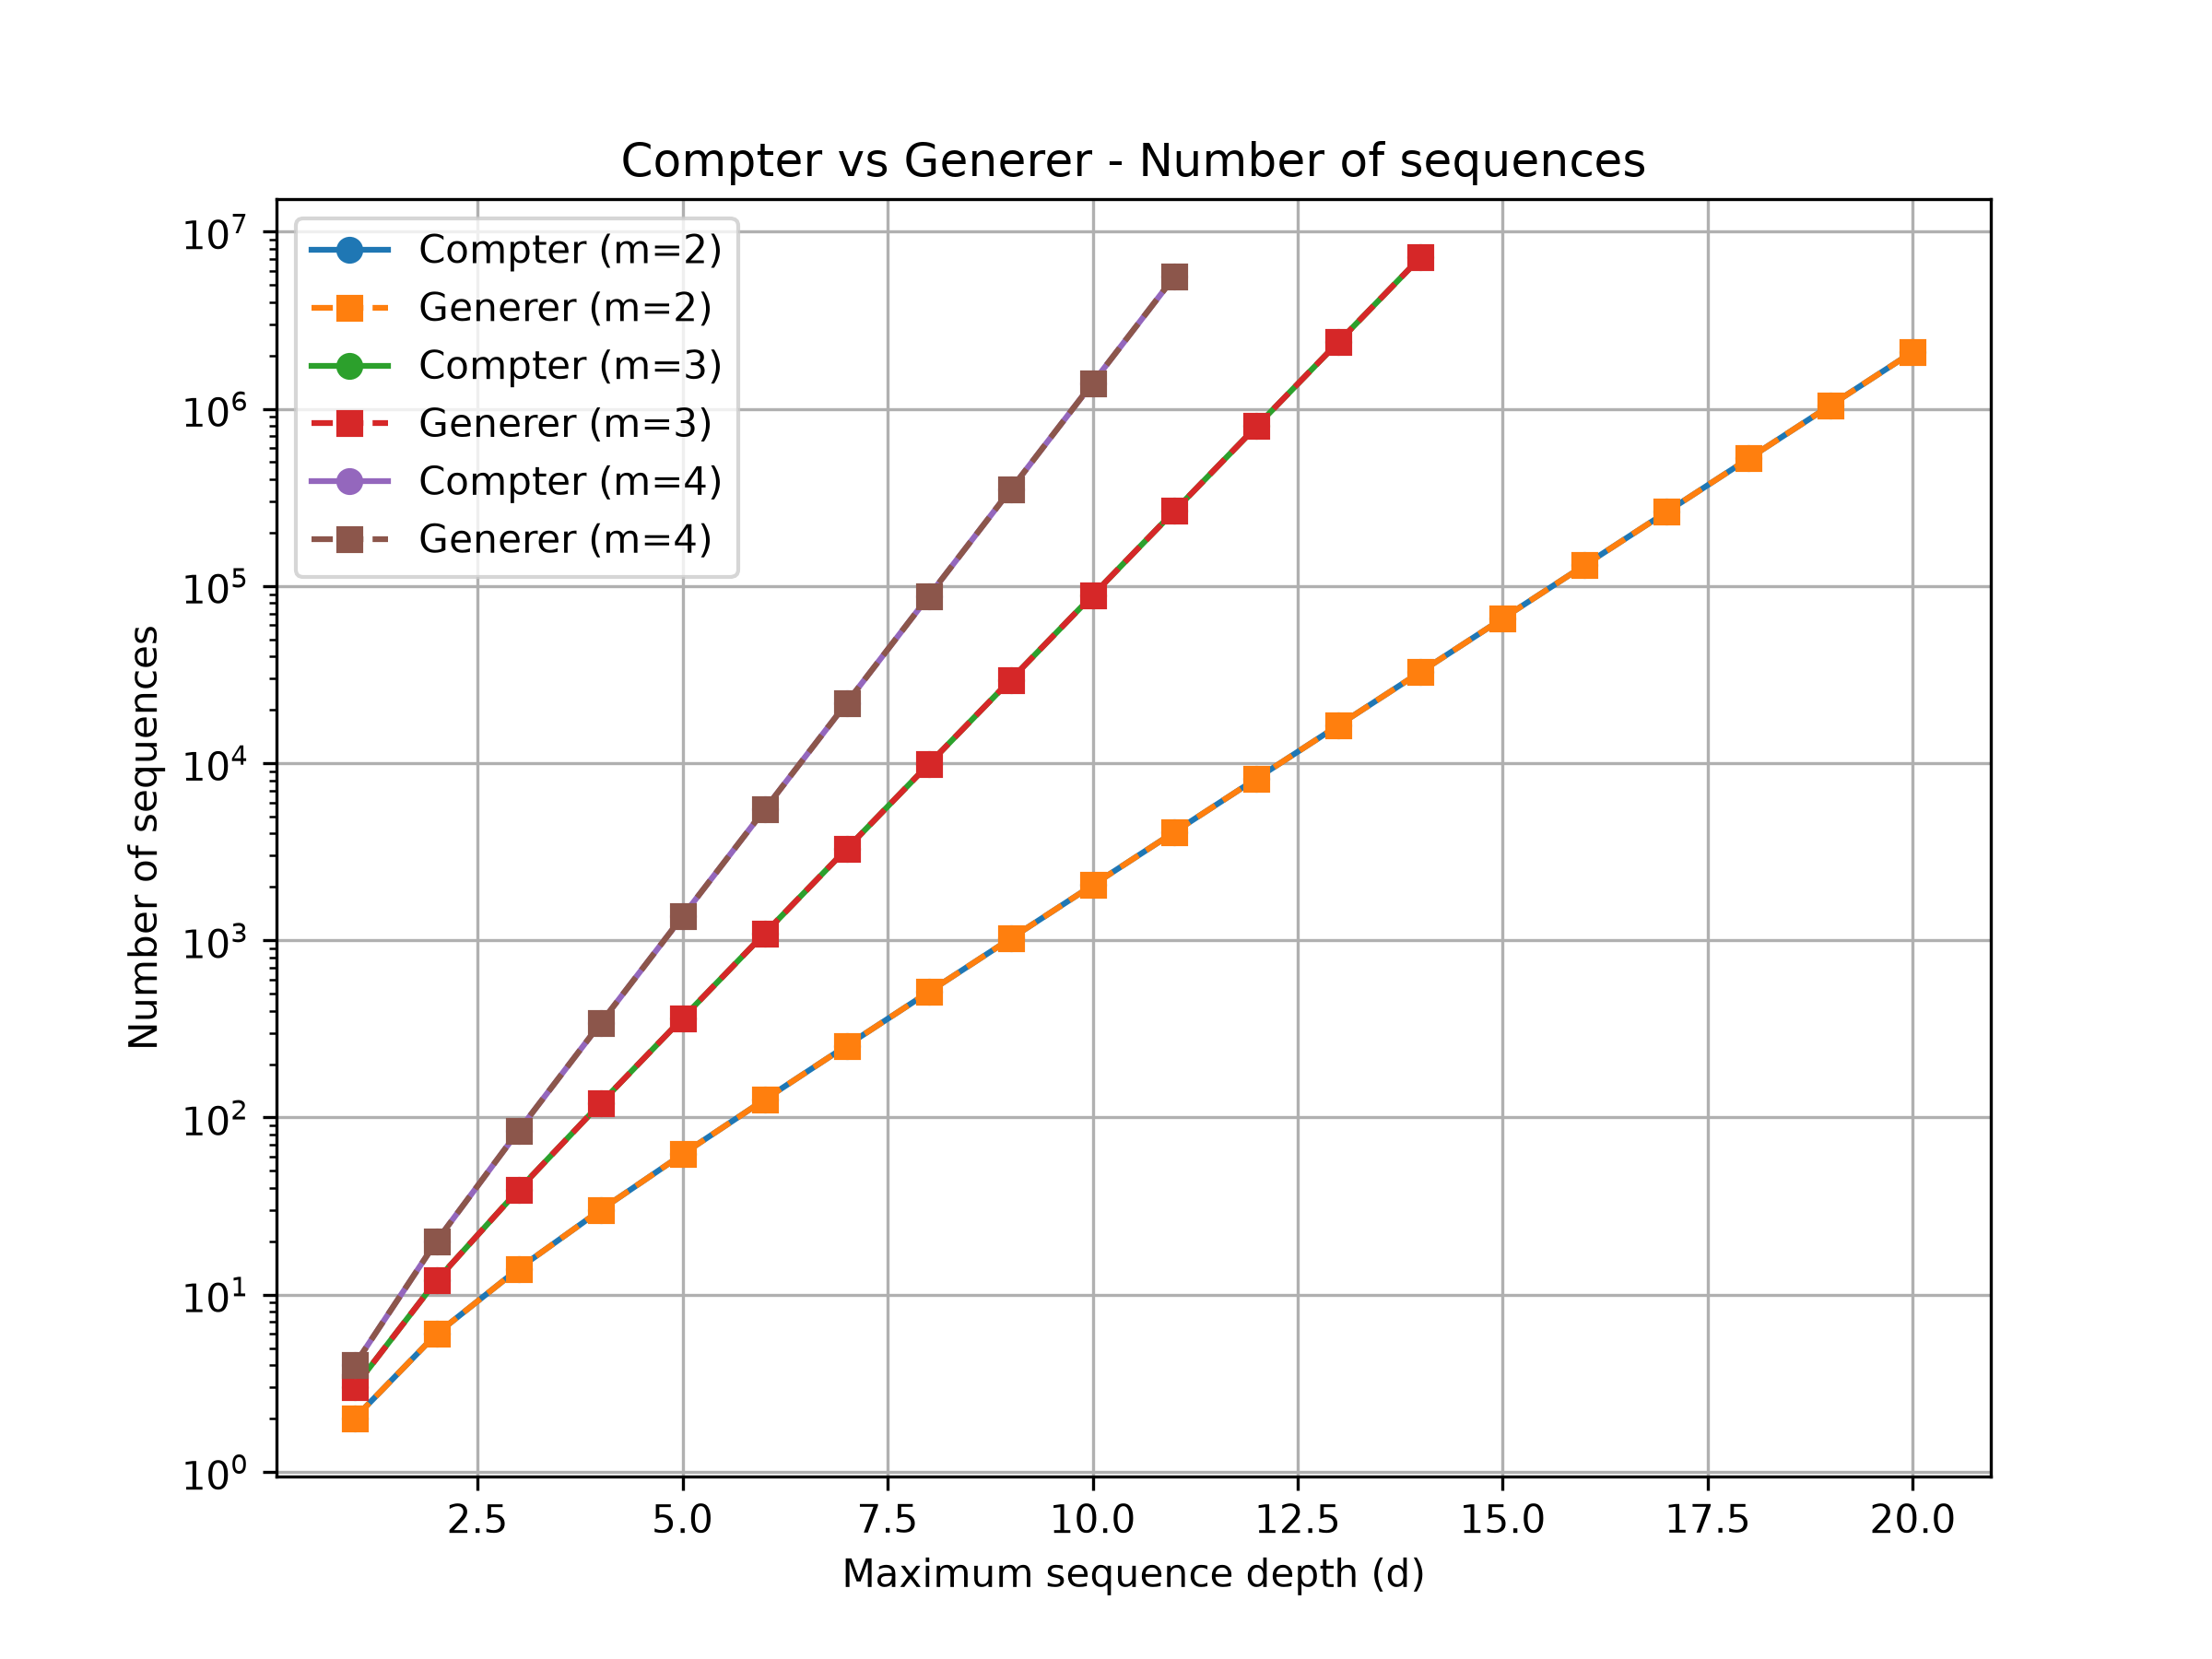
\includegraphics[width=1\textwidth]{images/compter-vs-generer-sequence-count.png}
		\caption{Comparison of the number of sequences generated}
		\label{fig:compter-vs-generer-sequence-count}
	\end{figure}
\end{minipage}
\hfill
\begin{minipage}[c]{0.45\textwidth}
	\centering
	\begin{figure}[H]
		\centering
		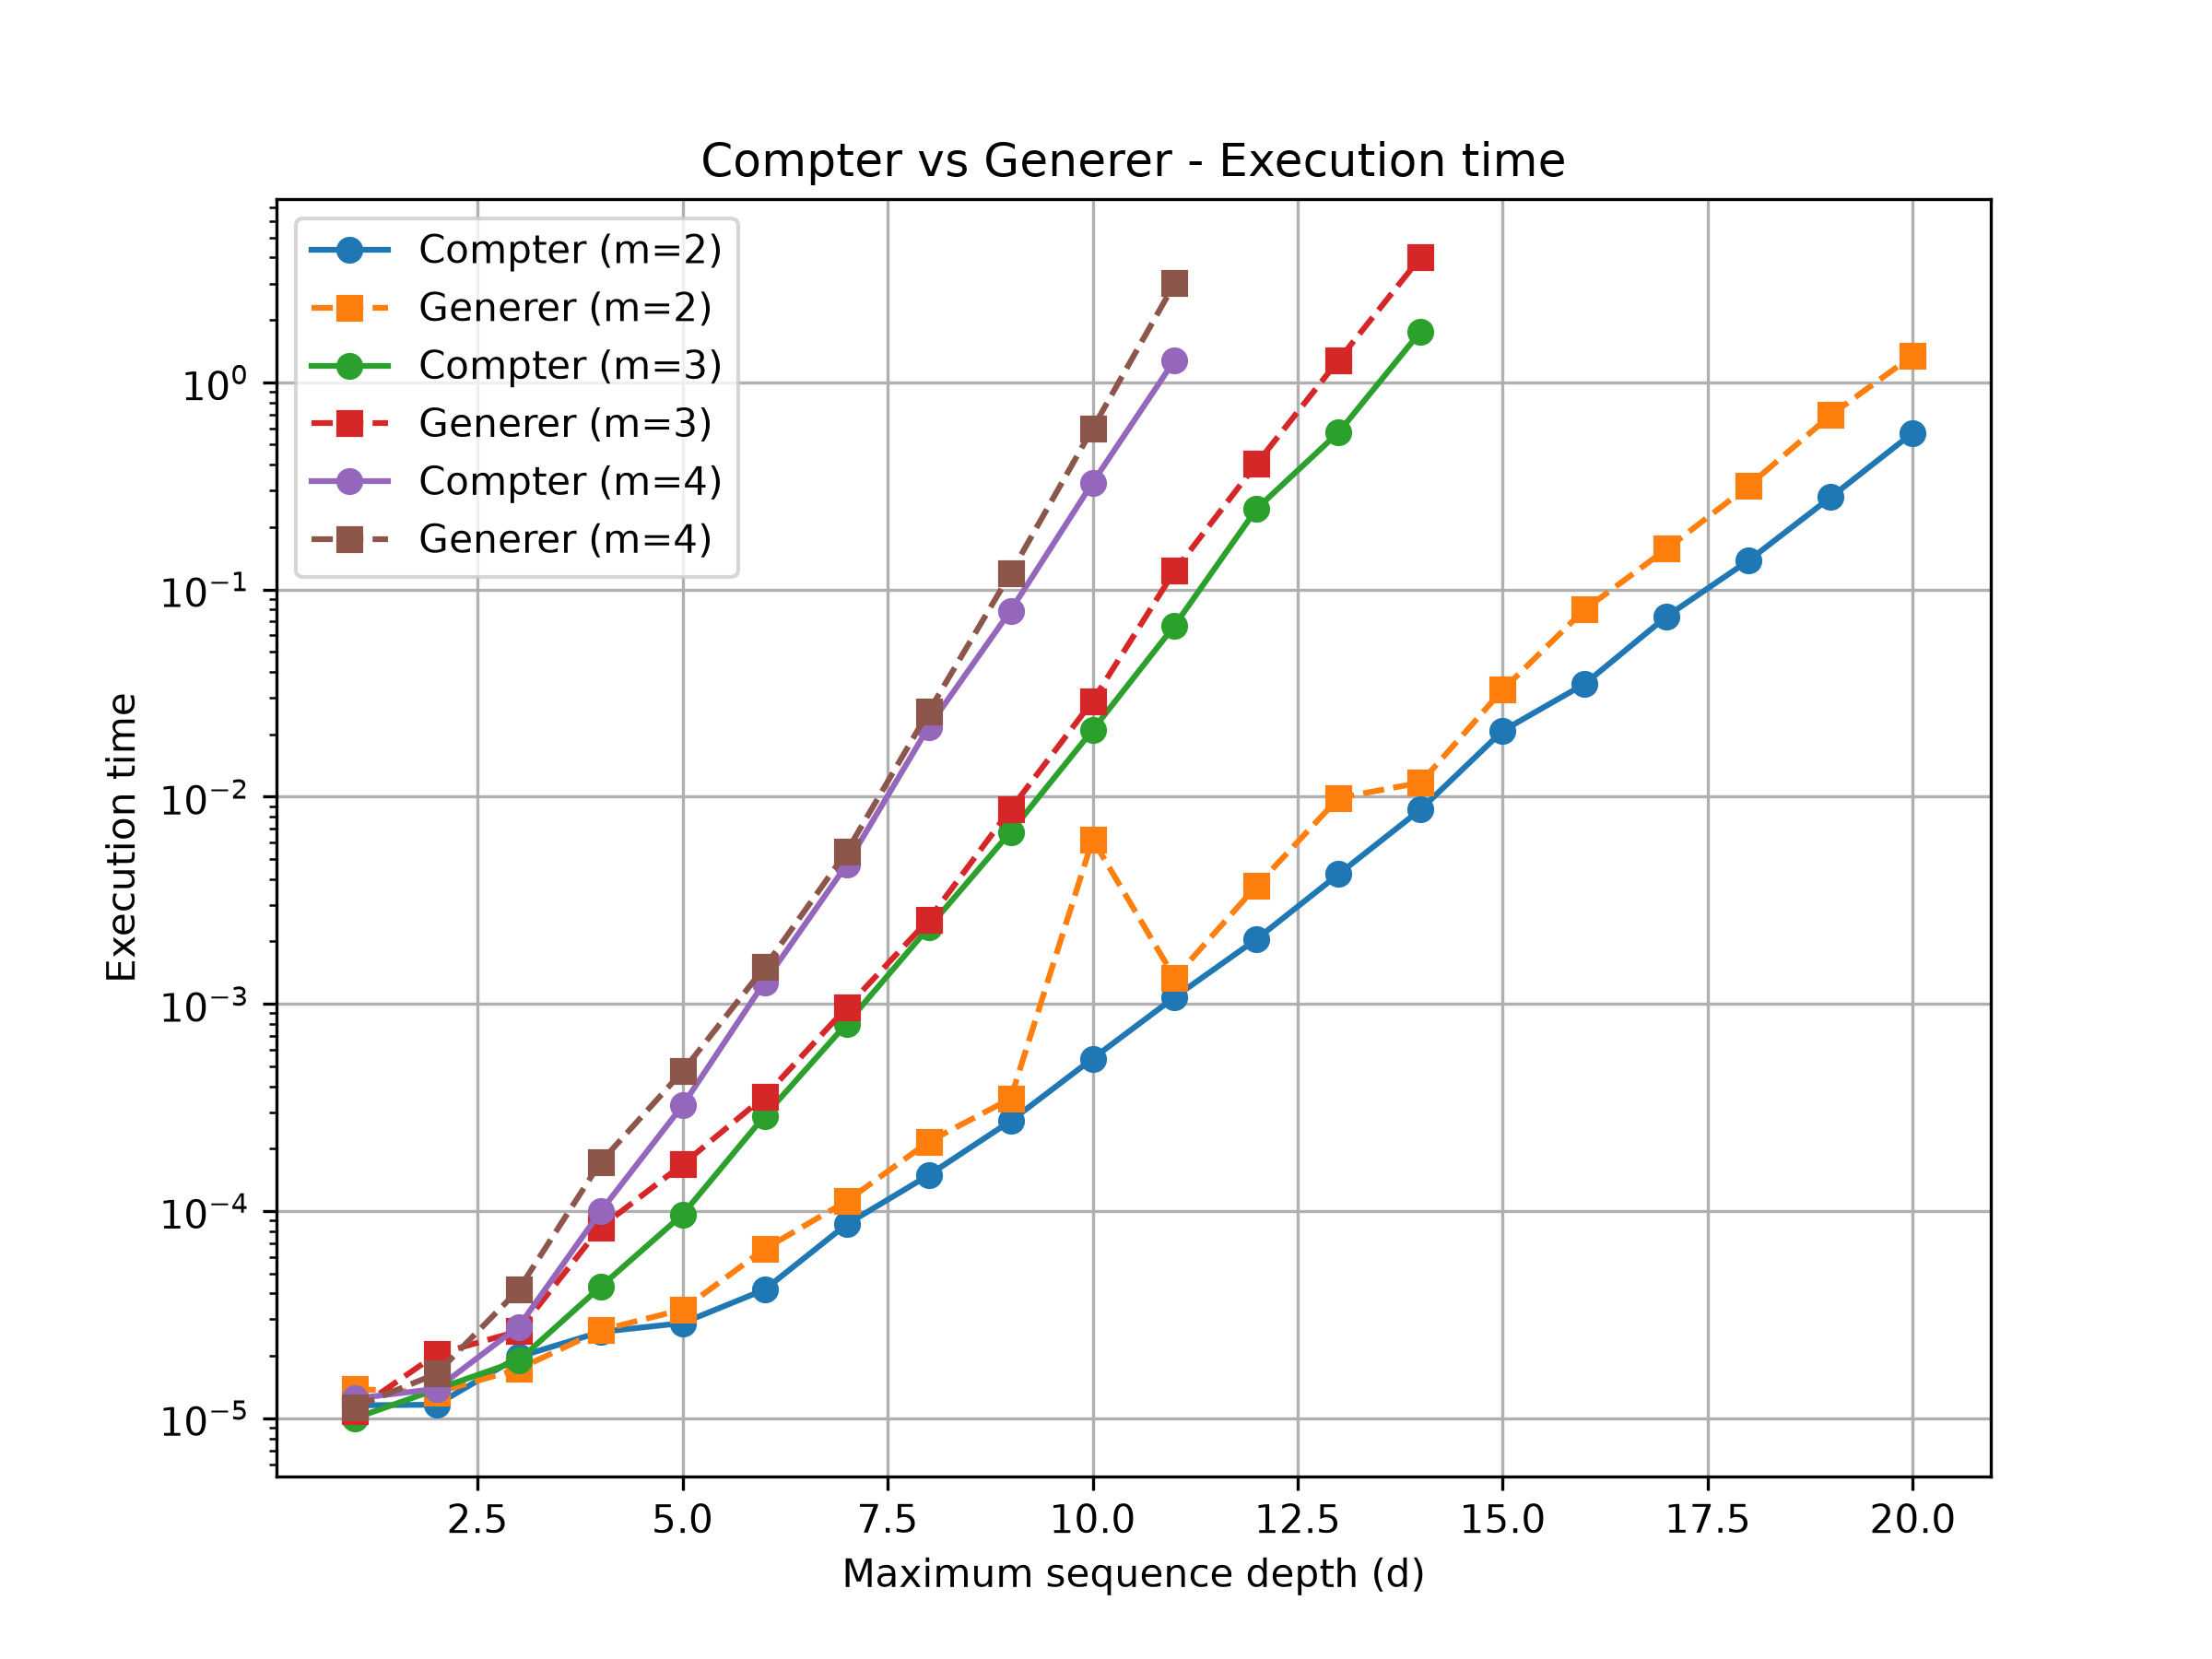
\includegraphics[width=1\textwidth]{images/compter-vs-generer-execution-time.png}
		\caption{Comparison of execution time (in seconds)}
		\label{fig:compter-vs-generer-execution-time}
	\end{figure}
\end{minipage}


\section*{Figures of the comparison between SPMF and our code}
\addcontentsline{toc}{section}{Figures of the comparison between SPMF and our code}

\begin{minipage}[c]{0.45\textwidth}
	\centering
	\begin{figure}[H]
		\centering
		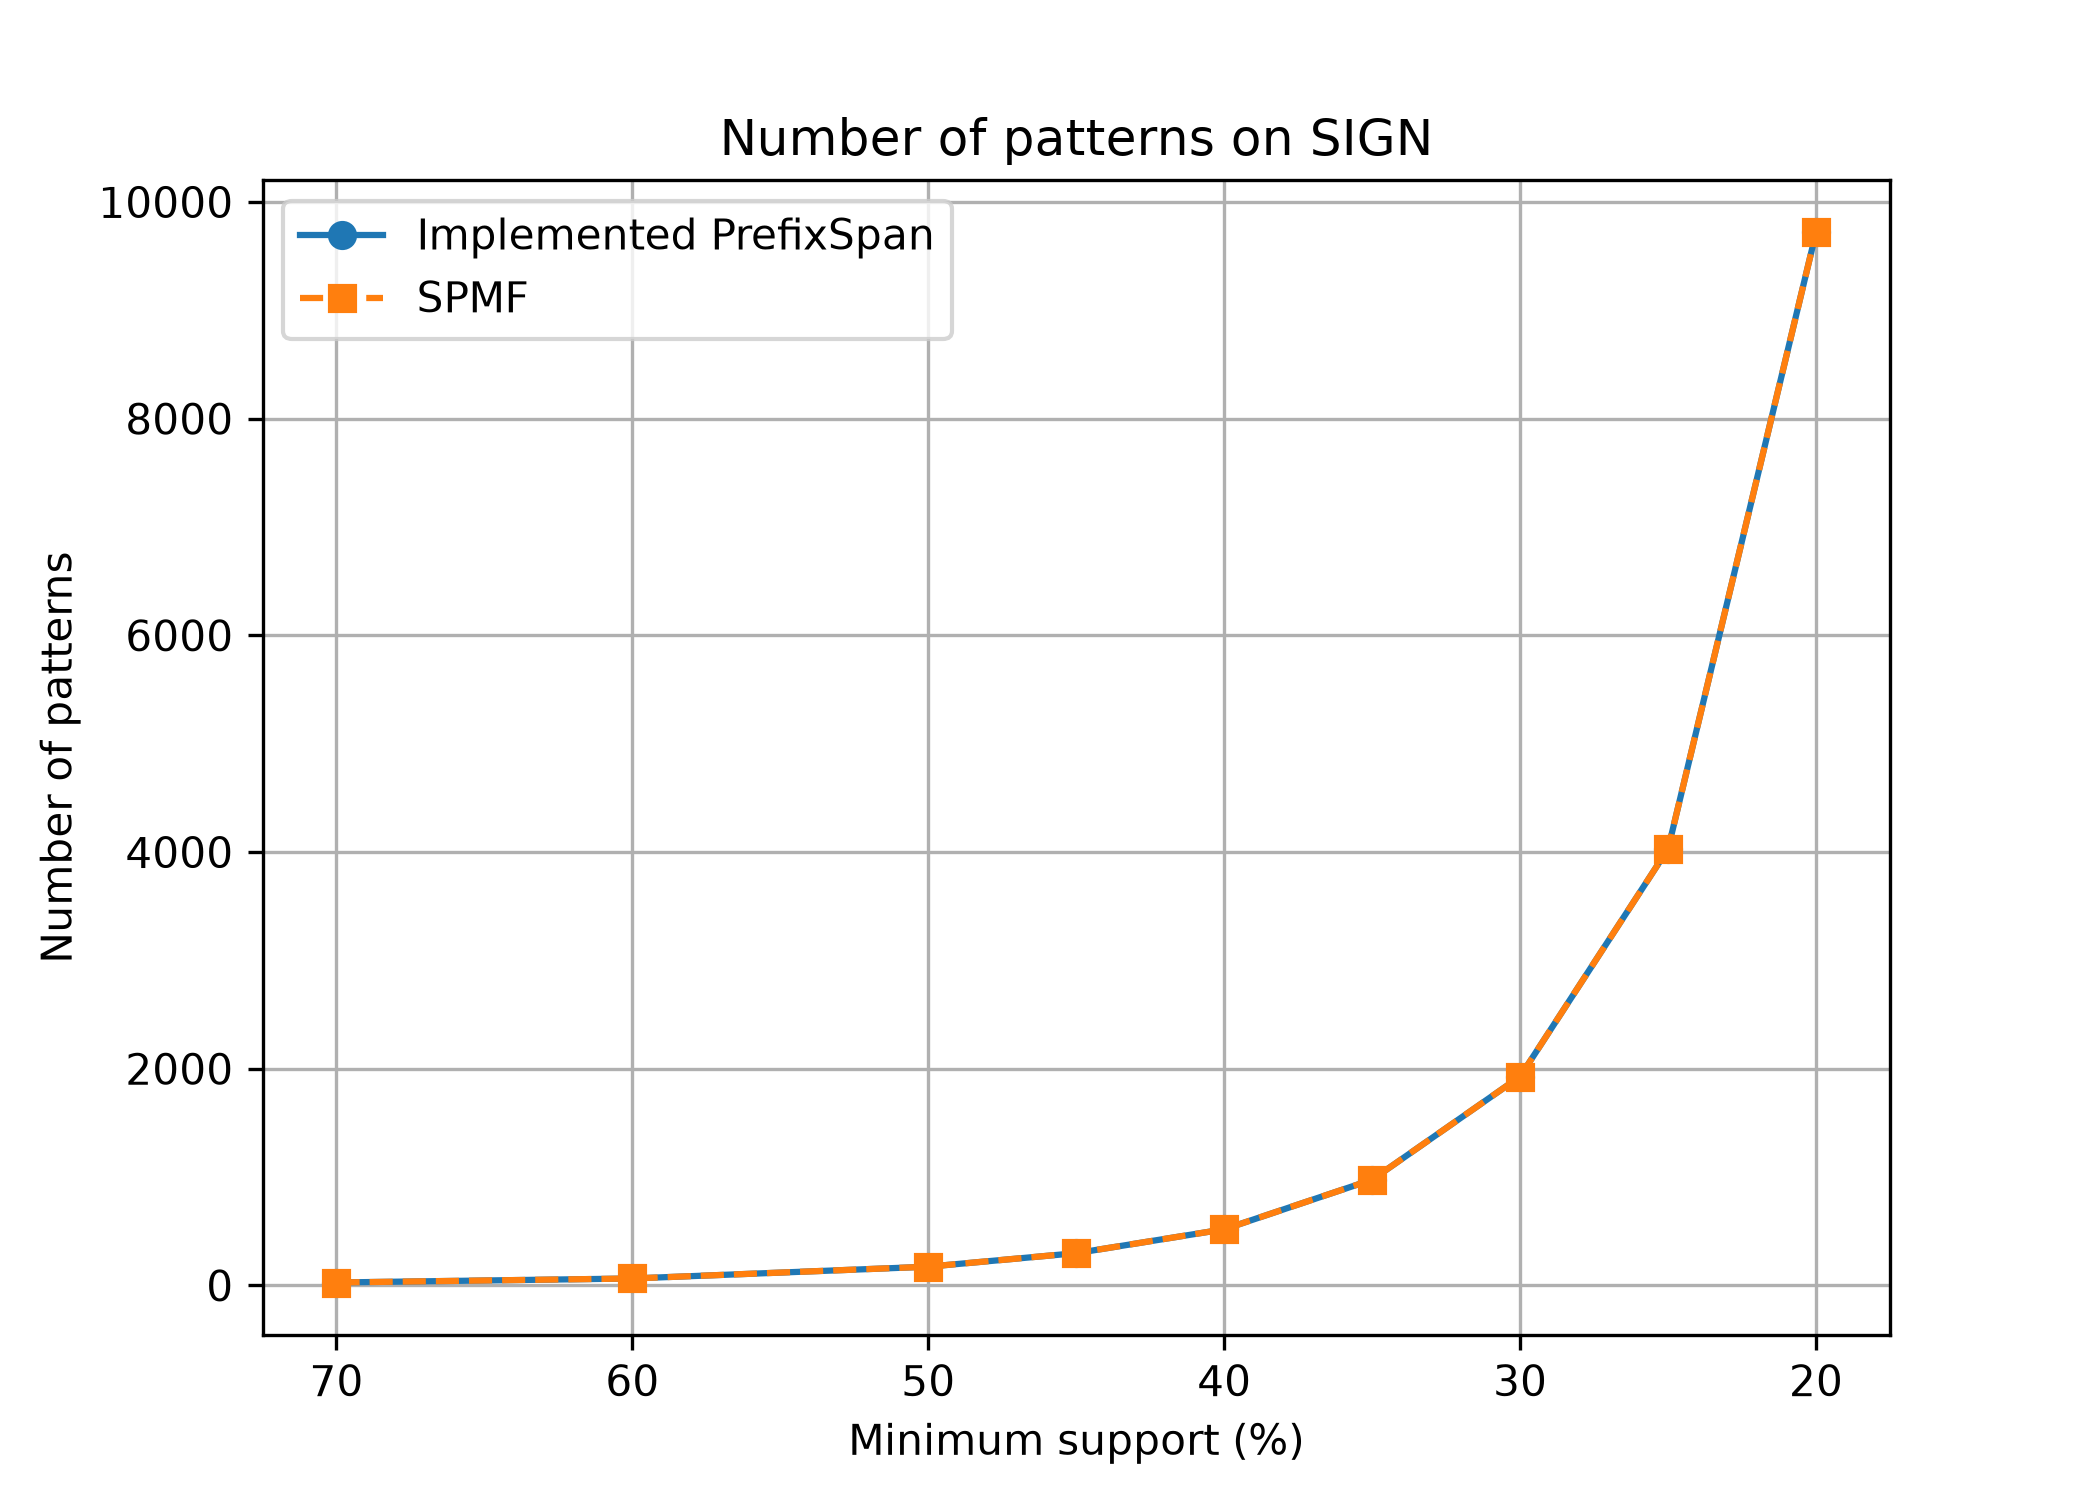
\includegraphics[width=1\textwidth]{images/sign-pattern-count.png}
		\caption{Number of sequences generated on the SIGN dataset}
		\label{fig:sign-pattern-count}
	\end{figure}
\end{minipage}
\hfill
\begin{minipage}[c]{0.45\textwidth}
	\centering
	\begin{figure}[H]
		\centering
		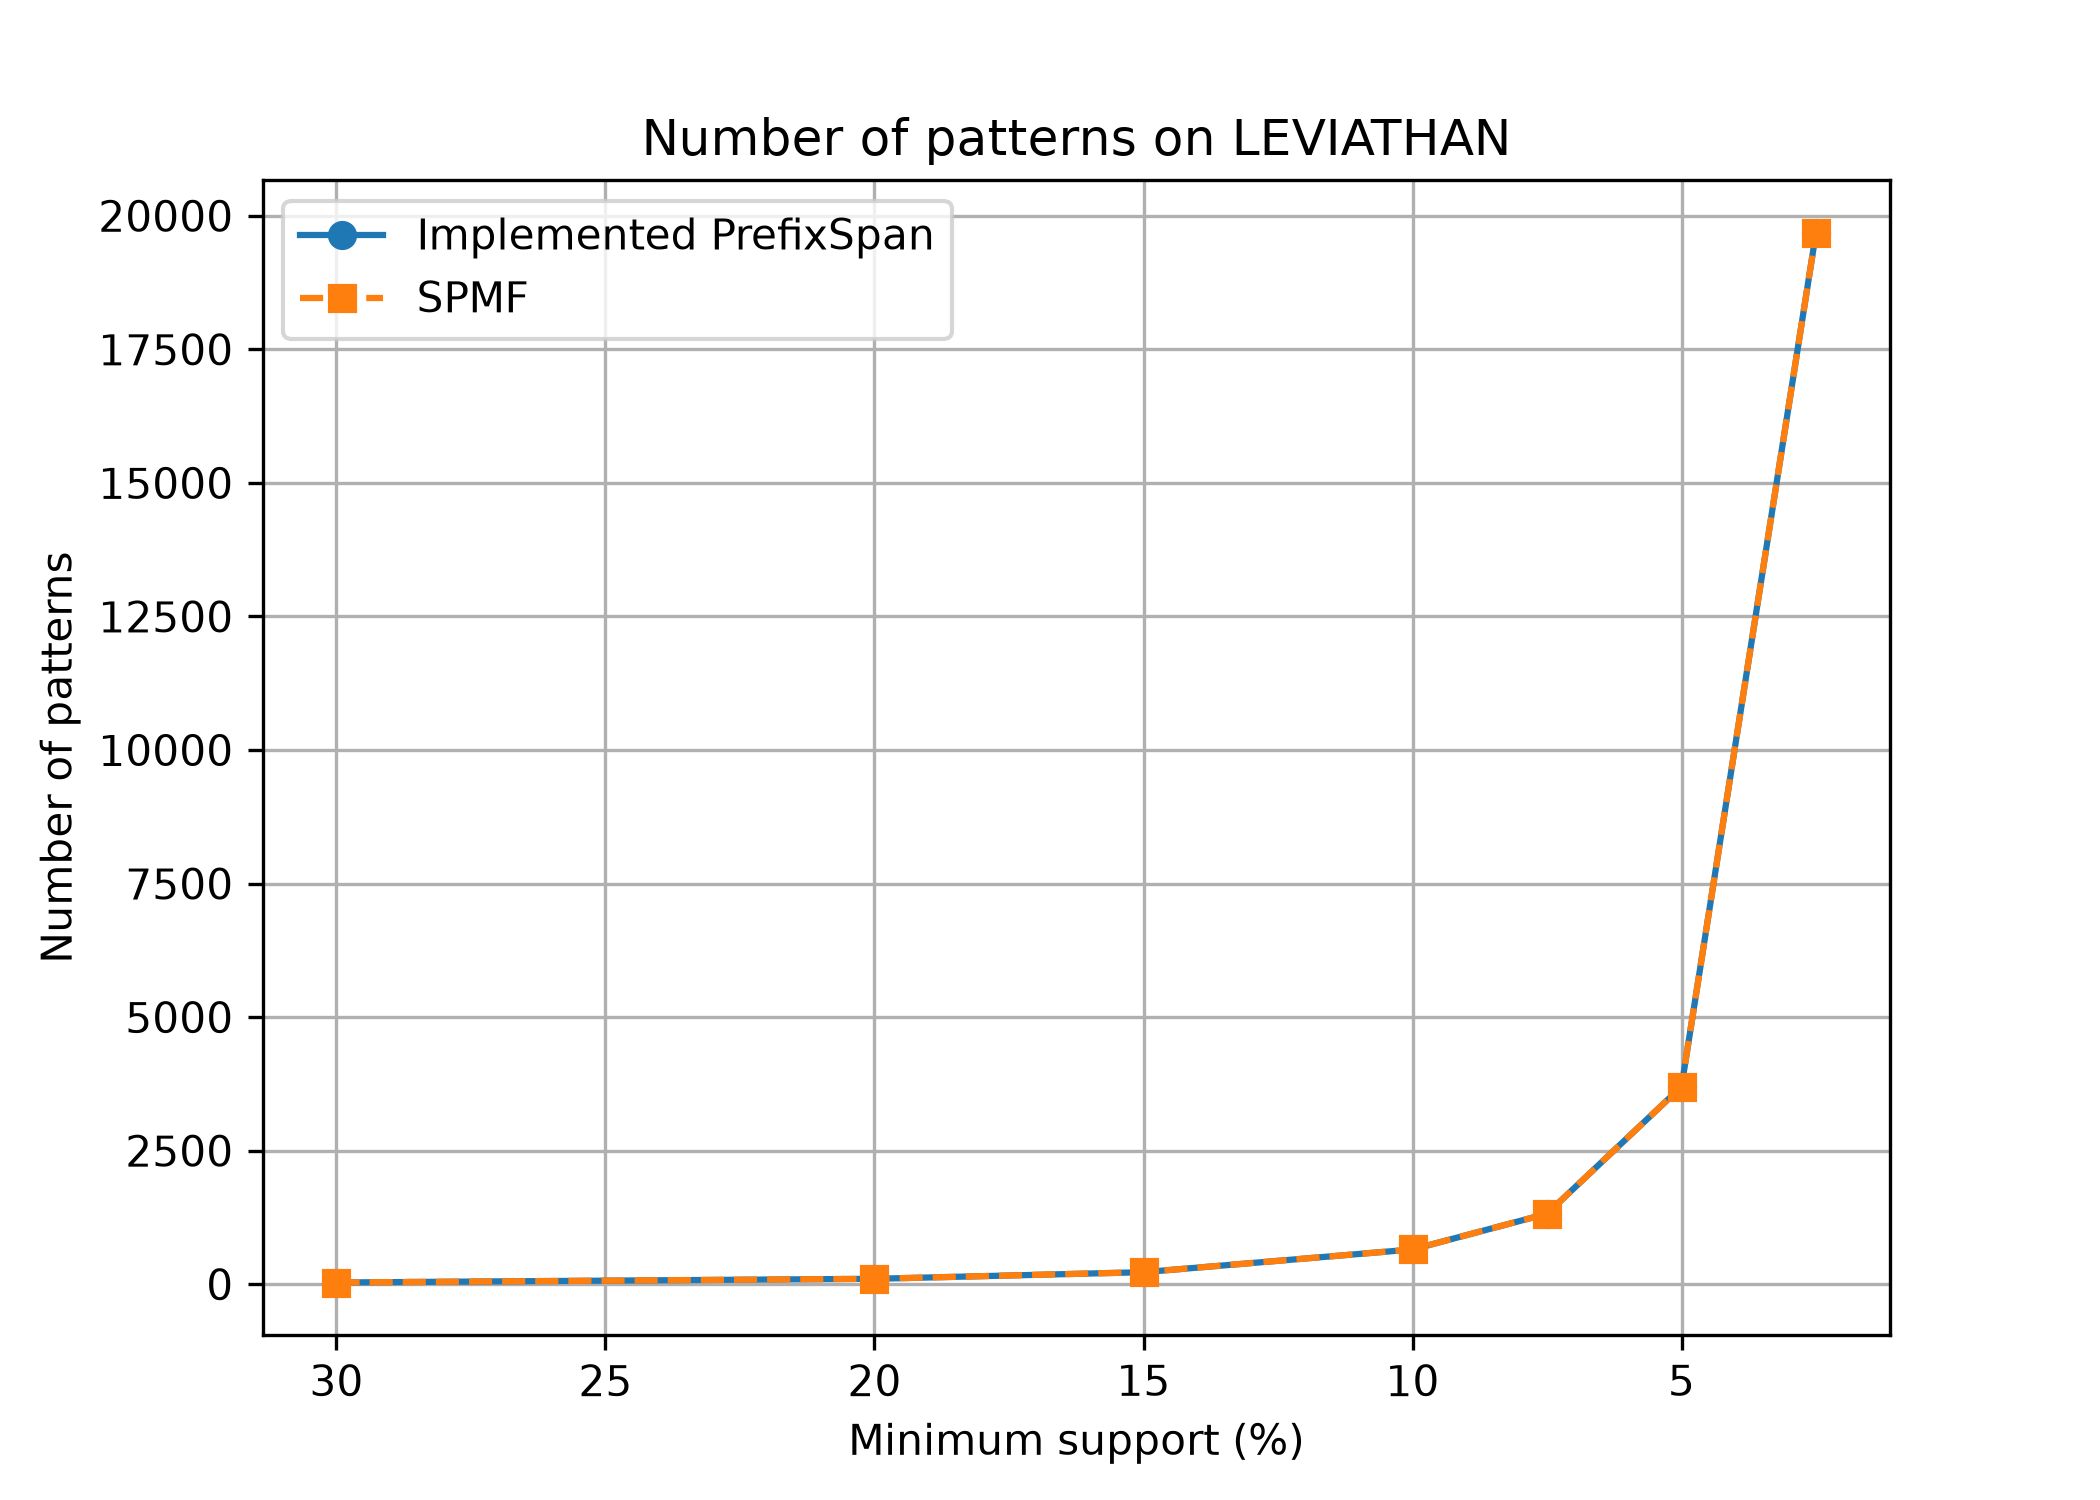
\includegraphics[width=1\textwidth]{images/leviathan-pattern-count.png}
		\caption{Number of sequences generated on the LEVIATHAN dataset}
		\label{fig:leviathan-pattern-count}
	\end{figure}
\end{minipage}

\begin{minipage}[c]{0.45\textwidth}
	\centering
	\begin{figure}[H]
		\centering
		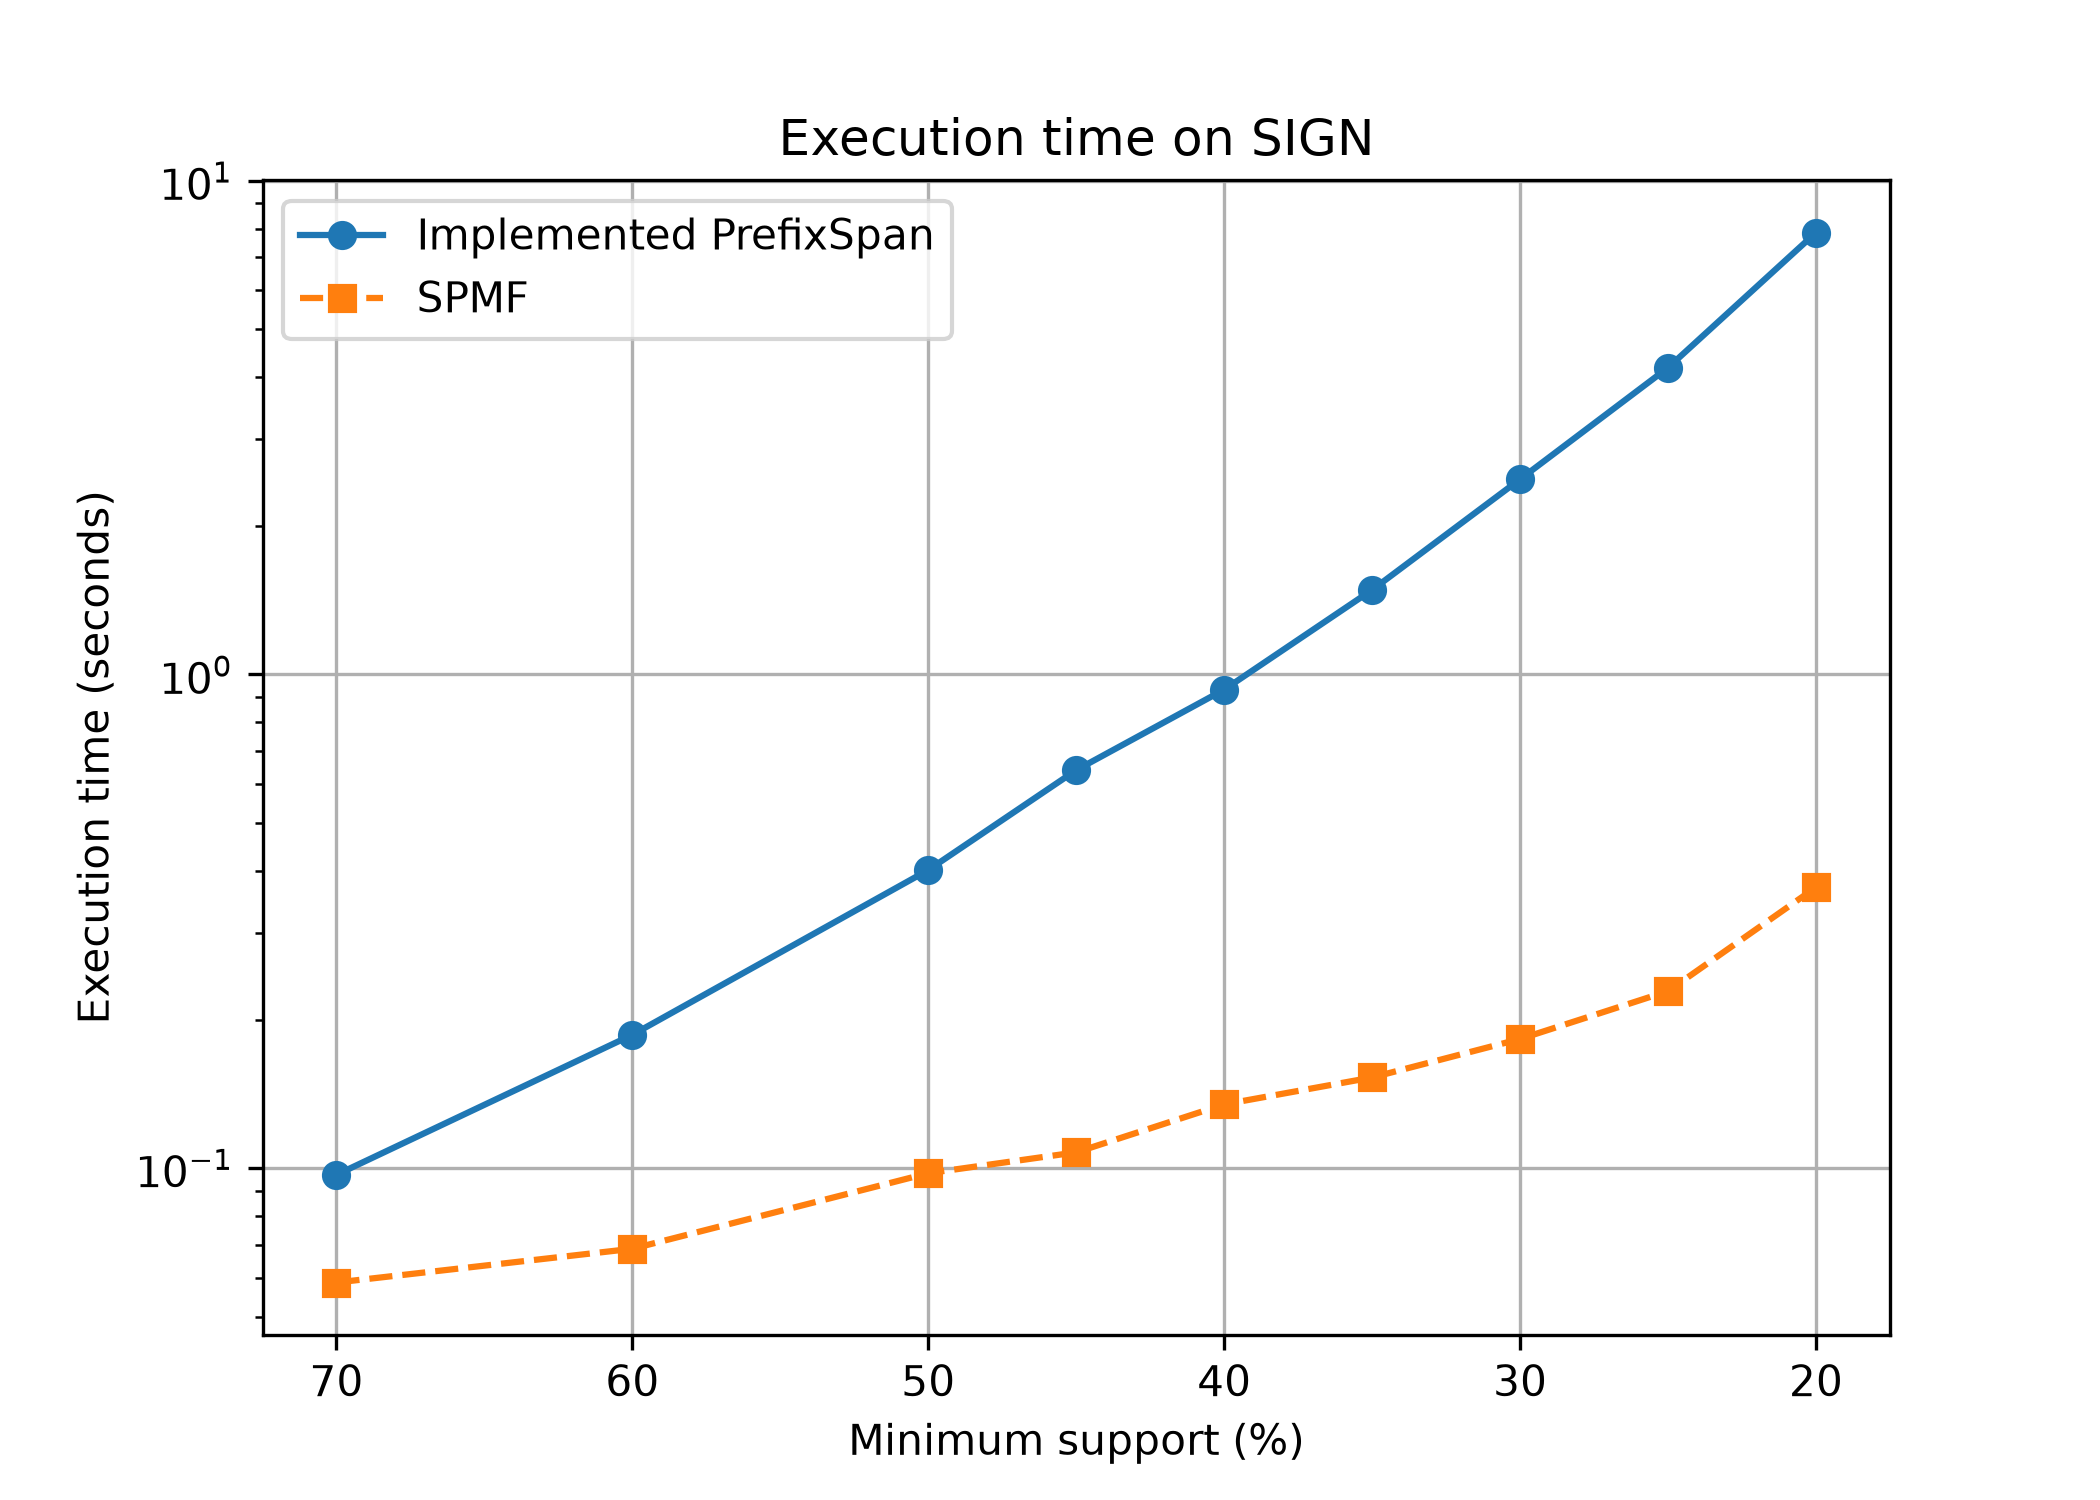
\includegraphics[width=1\textwidth]{images/sign-execution-time.png}
		\caption{Execution time on the SIGN dataset}
		\label{fig:sign-execution-time}
	\end{figure}
\end{minipage}
\hfill
\begin{minipage}[c]{0.45\textwidth}
	\centering
	\begin{figure}[H]
		\centering
		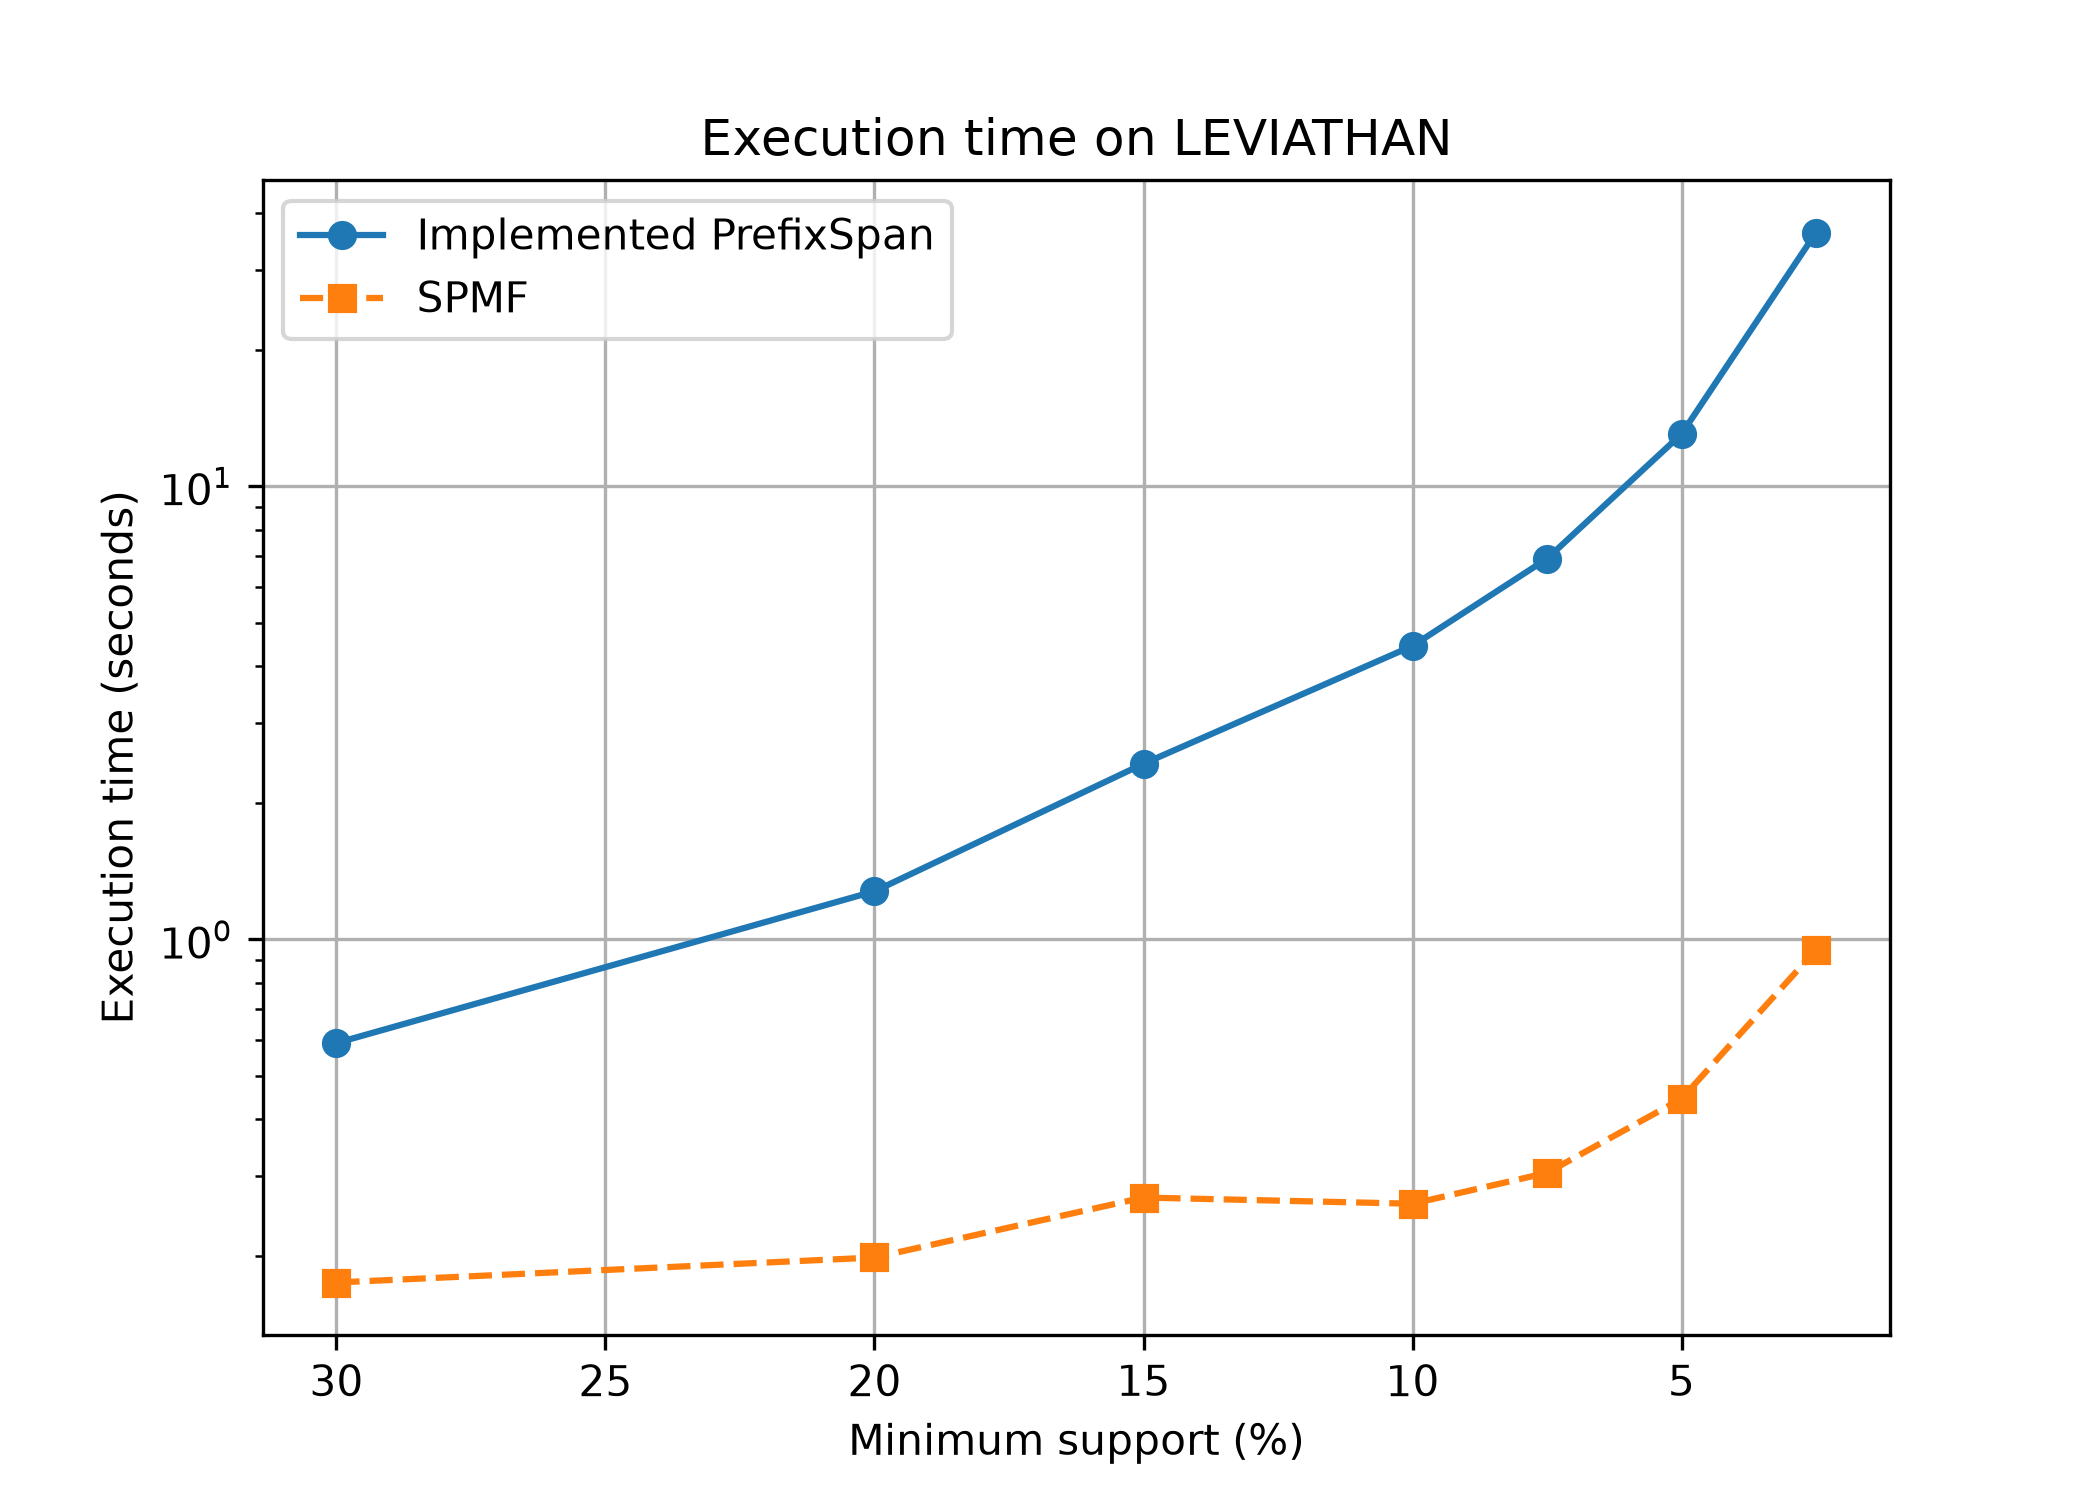
\includegraphics[width=1\textwidth]{images/leviathan-execution-time.png}
		\caption{Execution time on LEVIATHAN}
		\label{fig:leviathan-execution-time}
	\end{figure}
\end{minipage}


\section*{Table of Measurements}
\addcontentsline{toc}{section}{Table of Measurements}

\begin{table}[H]
	\centering
	\caption{Performance comparison between SPMF and our code for the SIGN dataset}
	\label{tab:performance-sign-spmf-code}
	\begin{tabular}{|r|r|r|r|r|r|}
		\hline
		\textbf{Minsup} & \textbf{PrefixSpan time} & \textbf{SPMF total time} & \textbf{SPMF internal time} & \textbf{Patterns} & \textbf{Speedup} \\ \hline
		70 & 0.096953 & 0.535673 & 0.058667 &   27 & 0.605101 \\ \hline
		60 & 0.186290 & 0.549740 & 0.068667 &   64 & 0.368602 \\ \hline
		50 & 0.401706 & 0.557264 & 0.097667 &  173 & 0.243130 \\ \hline
		45 & 0.640213 & 0.580376 & 0.107667 &  298 & 0.168173 \\ \hline
		40 & 0.931880 & 0.614480 & 0.134667 &  518 & 0.144511 \\ \hline
		35 & 1.483816 & 0.633412 & 0.152667 &  976 & 0.102888 \\ \hline
		30 & 2.486066 & 0.668858 & 0.182667 & 1928 & 0.073476 \\ \hline
		25 & 4.183554 & 0.719725 & 0.228333 & 4029 & 0.054579 \\ \hline
		20 & 7.857835 & 0.841723 & 0.370667 & 9718 & 0.047172 \\ \hline
	\end{tabular}
\end{table}

\begin{table}[H]
	\centering
	\caption{Performance comparison between SPMF and our code for the LEVIATHAN dataset}
	\label{tab:performance-leviathan-spmf-code}
	\begin{tabular}{|r|r|r|r|r|r|}
		\hline
		\textbf{Minsup} & \textbf{PrefixSpan time} & \textbf{SPMF total time} & \textbf{SPMF internal time} & \textbf{Patterns} & \textbf{Speedup} \\ \hline
		 30 &  0.590009 & 0.660830 & 0.174667 &    32 & 0.296040 \\ \hline
		 20 &  1.275746 & 0.691363 & 0.198333 &   101 & 0.155465 \\ \hline
		 15 &  2.439543 & 0.838718 & 0.269000 &   225 & 0.110266 \\ \hline
		 10 &  4.439838 & 0.763367 & 0.260667 &   651 & 0.058711 \\ \hline
		7.5 &  6.915959 & 0.807056 & 0.305000 &  1319 & 0.044101 \\ \hline
		  5 & 13.033781 & 0.923418 & 0.444333 &  3698 & 0.034091 \\ \hline
		2.5 & 36.301576 & 1.417876 & 0.947333 & 19687 & 0.026096 \\ \hline
	\end{tabular}
\end{table}


\section*{Specifications of the computer used for the measurements}
\addcontentsline{toc}{section}{Specifications of the computer used for the measurements}

\begin{itemize}
	\item \textbf{Processor:} Intel Core i5-6200U
	\item \textbf{RAM:} 8 GiB
	\item \textbf{Operating System:} Kubuntu 26.04 LTS
\end{itemize}


\section*{References}
\addcontentsline{toc}{section}{References}

\begin{itemize}
	\item J. Pei, J. Han, B. Mortazavi-Asl, H. Pinto, Q. Chen, U. Dayal, M.-C. Hsu, « PrefixSpan: Mining Sequential Patterns Efficiently by Prefix-Projected Pattern Growth », Proceedings of the 17th International Conference on Data Engineering (ICDE), 2001, p. 215–224.
	\item J. Pei, J. Han, B. Mortazavi-Asl, J. Wang, H. Pinto, Q. Chen, U. Dayal, M.-C. Hsu, « Mining Sequential Patterns by Pattern-Growth: The PrefixSpan Approach », IEEE Transactions on Knowledge and Data Engineering, 16(11), 2004, p. 1424–1440.
	\item P. Fournier-Viger et al., « SPMF: A Java Open-Source Pattern Mining Library », Journal of Machine Learning Research, 15, 2014, p. 3389–3393. Site : \url{https://www.philippe-fournier-viger.com/spmf/}.
	\item Documentation SPMF — PrefixSpan: \url{https://www.philippe-fournier-viger.com/spmf/PrefixSpan.php}.
	\item SPMF Datasets: \url{https://www.philippe-fournier-viger.com/spmf/datasets.php}.
\end{itemize}

\end{document}
